\begin{enumerate}[label=\thesubsection.\arabic*,ref=\thesubsection.\theenumi]
    \item In a $\triangle ABC$, $\angle A=90\degree$ and $AD$ is an altitude. Complete the relation
    $$\frac{BD}{BA} = \frac{AB}{(\dots)}.$$
    \hfill (1980)
    
    \item $ABC$ is a triangle, $P$ is a point on $AB$, and $Q$ is point on $AC$ such that $\angle AQP = \angle ABC$. Complete the relation
	    $$\frac{ar\brak{\triangle APQ}}{ar\brak{\triangle ABC}} =\frac{(\dots)}{AC^2}$$
    \hfill (1980)
    
    \item $ABC$ is a triangle with $\angle B $ greater than $\angle C$.
    $D$ and $E$ are the points on $BC$ such that $AD$ is perpendicular to $BC$ and $AE$ is the bisector of angle $A$. Complete the relation
    $$\angle DAE = \frac{1}{2} [( ) - \angle C].$$
    \hfill (1980)
    \item The set of all real numbers $a$ such that $a^2 + 2a, 2a + 3$ and $a^2 + 3a + 8$ are the sides of a triangle is \rule{1cm}{0.1pt}.
    \hfill (1985)
    \item In   $\triangle ABC$, if $\cot A, \cot B, \cot C$ are in A.P., then $a^2,b^2,c^2$ are in \rule{1cm}{0.1pt} progression 

	    \hfill (1985)
    \item If in the $\triangle ABC$, 
	    $$\frac{2\cos A}{a} + \frac{2\cos B}{b} + \frac{2\cos C}{c} = \frac{a}{bc} +  \frac{b}{ac},$$ 
		then the value of the angle $A$ is \rule{1cm}{0.1pt} degrees. \hfill (1993)
    \item In the $\triangle ABC$, $AD$ is the altitude from $A$. Given $b>c$, $\angle C=23 \degree$ and $AD = \frac{abc}{b^2 - c^2}$ then $\angle B =  \rule{1cm}{0.1pt}$.\hfill (1994)
%
\item In a $\triangle{ABC}$, medians $AD$ and $BE$ are drawn. If $AD=4,\angle{DAB}=\frac{\pi}{6}$  and $\angle{ABE}=\frac{\pi}{3}$, then the area of the $\triangle{ABC}$ is \hfill\brak{2003}
\begin{multicols}{4}
\begin{enumerate}
        \item $\frac{64}{3}$                    
        \item $\frac{8}{3}$ 
        \item $\frac{16}{3}$ 
        \item $\frac{32}{3\sqrt{3}}$
\end{enumerate}
\end{multicols} 
%
\item If in $\triangle{ABC},a\cos^2\brak{\frac{{C}}{2}} + c\cos^2\brak{\frac{{A}}{2}} = \frac{3b}{2},$ then the sides $a,b\text{ and }c$ \hfill\brak{2003}
\begin{multicols}{4}
\begin{enumerate}
        \item satisfy $a+b=c$                    
        \item are in A.P. 
        \item are in G.P. 
        \item are in H.P.
\end{enumerate}
\end{multicols} 
%
\item The sides of a triangle are $\sin\alpha,\cos\alpha$ and $ \sqrt{1+\sin\alpha\cos\alpha}$ for some $0<\alpha<\frac{\pi}{2}.$ Then the greatest angle of the triangle is \hfill\brak{2004}
\begin{multicols}{4}
\begin{enumerate}
        \item $150\degree$                    
        \item $90\degree$ 
        \item $120\degree$
        \item $60\degree$
\end{enumerate}
\end{multicols} 
%
\item In a $\triangle{ABC}$, let $\angle{C}=\frac{\pi}{2}.$ If $r$ is the inradius and $R$ is the circumradius of the $ \triangle{ABC},$ then $2\brak{R+r}$ equals \hfill\brak{2005}
\begin{multicols}{4}
\begin{enumerate}
        \item $b+c$                    
        \item $a+b$ 
        \item $a+b+c$ 
        \item $c+a$
\end{enumerate}
\end{multicols} 
%
\item If in a $\triangle ABC,$ the altitudes from the vertices ${A,B,C}$ on opposite sides are in H.P., then $\sin {A},\sin {B},\sin {C}$ are in \hfill\brak{2005}
\begin{multicols}{4}
\begin{enumerate}
        \item $G.P.$                    
        \item $A.P.$ 
        \item $A.P.-G.P.$ 
        \item $H.P.$
\end{enumerate}
\end{multicols} 
%
    \item There exists a $\triangle ABC$ satisfying the conditions
    \hfill{(1986)}
\begin{multicols}{2}
    \begin{enumerate}
    	\item $b\sin{A} = a, A <\pi/2$
    	\item $b\sin{A} > a, A >\pi/2$
    	\item $b\sin{A} > a, A <\pi/2$
    	\item $b\sin{A} < a, A <\pi/2$, $b > a$
    	\item $b\sin{A} < a, A >\pi/2$, $b = a$
    \end{enumerate}
\end{multicols} 
    \item In a triangle, the lengths of two larger sides are $10$ and $9$ respectively. If the angles are in AP, Then length of third side is
    \hfill{(1987)}
    \begin{multicols}{2}
    	\begin{enumerate}
    		\item $5-\sqrt{6}$ 
    		\item $3\sqrt{3}$
    		\item $3$
    		\item $5+\sqrt{6}$ 
    		\item none
    	\end{enumerate}
    \end{multicols}
    \item If in a $\triangle PQR$, $\sin{P}, \sin{Q}, \sin{R}$ are in AP, then
    \hfill{(1998)}
    \begin{multicols}{2}
    \begin{enumerate}
    	\item The altitudes are in AP
    	\item The altitudes are in HP
    	\item The medians are in GP
    	\item The medians are in AP
    \end{enumerate}
    \end{multicols}
    \item In $\triangle ABC$, internal angle bisector of $\angle A$ meets side $BC$ in ${D}$. $DE \perp AD$ meets $AC$ in ${E}$ and $AB$ in ${F}$. Then
    \hfill{(2006)}
    \begin{multicols}{2}
    \begin{enumerate}
    	\item $AE$ is HM of $b \text{ and } c$
    	\item $AD$ = ${\frac{2bc}{b+c}}\cos{\frac{A}{2}}$
    	\item $EF$ = ${\frac{4bc}{b+c}}\sin{\frac{A}{2}}$
    	\item $\triangle AEF$ is isosceles
    \end{enumerate}
    \end{multicols}
    \item Let $ABC$ be a triangle such that $\angle ACB = \pi/6$ and let $a,b \text{ and } c$ denote lengths of the sides opposite to ${A}$,${B} \text{ and } {C}$ respectively. The value(s) of $x$ for which $a = x^{2}+x+1, b = x^{2}-1, c = 2x+1$ is (are)
    \hfill{(2010)}
    \begin{multicols}{4}
    	\begin{enumerate}
    		\item $-(2+\sqrt{3})$
    		\item $1+\sqrt{3}$
    		\item $2+\sqrt{3}$
    		\item $4\sqrt{3}$
    	\end{enumerate}
    \end{multicols}
    \item If the bisector of the angle $P$ of a $\triangle PQR$ meets $QR$ in $S$, then \hfill (1979)
\begin{multicols}{2}
    \begin{enumerate}
        \item $QS = SR$
        \item $QS : SR = PR : PQ$
        \item $QS : SR = PQ : PR$
        \item None of these \hfill 
    \end{enumerate}
\end{multicols}
    \item In the $\triangle ABC$, angle $A$ is the greater than angle $B$. If the measures of the angles $A$ and $B$ satisfies the equation $3\sin x - 4 \sin^3 x - k = 0, 0<k<1$, then the measure of the angle $C$ is 
		\hfill (1985)
	    \begin{multicols}{4}
	    \begin{enumerate}
     \item $\frac{\pi}{3}$
     \item $\frac{\pi}{2}$
     \item $\frac{2\pi}{3}$
     \item $\frac{5\pi}{6}$ 
\end{enumerate}
	    \end{multicols}
    \item If the lengths of the sides of a triangle are $3,5,7$ then the largest angle of the triangle is
		\hfill (1986)
	    \begin{multicols}{4}
	    \begin{enumerate}
     \item $\frac{\pi}{2}$
     \item $\frac{5\pi}{6}$
     \item $\frac{2\pi}{3}$
     \item $\frac{3\pi}{4}$ 
	    \end{enumerate}
	    \end{multicols}
\item In a $\triangle ABC$, $\angle B = \frac{\pi}{3}$ and $\angle C = \frac{\pi}{4}$. Let ${D}$ divide $BC$ internally in the ratio $1\colon3$ then $\frac{\sin\angle BAD}{\sin \angle CAD}$ is equal to
\hfill (1995)
	    \begin{multicols}{4}
\begin{enumerate}
\item $\frac{1}{\sqrt6}$
\item $\frac{1}{3}$
\item $\frac{1}{\sqrt3}$
\item $\sqrt{\frac{2}{3}}$
\end{enumerate}
	    \end{multicols}
%
\item In a $\triangle ABC, 2ac\sin\frac{1}{2}\brak{A-B+C} = $
\hfill (2000)
	    \begin{multicols}{2}
\begin{enumerate}
\item $a^2 + b^2 - c^2$
\item $c^2 + a^2 - b^2$
\item $b^2 - c^2 - a^2$
\item $c^2 - a^2 - b^2$
\end{enumerate}
	    \end{multicols}
%
\item In a $\triangle ABC$, let $\angle C = \frac{\pi}{2}$. If ${r}$ is the inradius and ${R}$ is the circumradius of the triangle, then $2\brak{r+R}$ is equal to
\hfill (2000)
\begin{multicols}{4}
\begin{enumerate}
\item $a+b$
\item $b+c$
\item $c+a$
\item $a+b+c$
\end{enumerate}
\end{multicols}
\item If the angles of a triangle are in the ratio $4\colon1\colon1$, then the ratio of the longest side to the perimeter is
\hfill (2003)
\begin{multicols}{4}
\begin{enumerate}
\item $\sqrt{3}\colon2+\sqrt{3}$
\item $1\colon6$
\item $1\colon2+\sqrt{3}$
\item $2\colon3$
\end{enumerate}
\end{multicols}
%
\item The sides of a triangle are in the ratio $1\colon\sqrt{3}\colon2$, then the angles of the triangle are in the ratio
\hfill (2004)
\begin{multicols}{2}
\begin{enumerate}
\item $1\colon3\colon5$
\item $2\colon3\colon4$
\item $3\colon2\colon1$
\item $1\colon2\colon3$
\end{enumerate}
\end{multicols}
%
\item In an equilateral triangle, $3$ coins of radii $1$ unit each are kept so they touch each other and also the sides of the triangle. Area of the triangle is 
\hfill (2005)
\begin{figure}[htp]
    \centering
    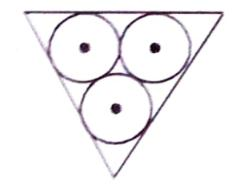
\includegraphics[width=0.75\columnwidth]{figs/figure.png}
    \label{fig:figure}
\end{figure}
\begin{multicols}{4}
\begin{enumerate}
\item $4+2\sqrt{3}$
\item $6+4\sqrt{3}$
\item $12+\frac{7\sqrt{3}}{4}$
\item $3+\frac{7\sqrt{3}}{4}$
\end{enumerate}
\end{multicols}
%
\item In a $\triangle ABC$, $a, b, c$  are the lengths of its sides and $A, B, C$ are the angles of $\triangle ABC$. The correct relation is given by
\hfill (2005)
\begin{multicols}{2}
\begin{enumerate}
\item $\brak{b-c} \sin \brak{\frac{B-C}{2}} = a \cos \brak{\frac{A}{2}}$
\item $\brak{b-c} \cos \brak{\frac{A}{2}} = a \sin \brak{\frac{B-C}{2}}$
\item $\brak{b-c} \sin \brak{\frac{B+C}{2}} = a \cos \brak{\frac{A}{2}}$
\item $\brak{b-c} \cos \brak{\frac{A}{2}} = a \sin \brak{\frac{B+C}{2}}$
\end{enumerate}
\end{multicols}
%
\item If the angles $A, B$ and $C$ of a triangle are in an arithmetic progression and if ${a}, {b}$ and ${c}$ denote the lengths of the sides opposite to $A, B$ and $C$ respectively, then the value of the expression $\frac{a}{c}\sin 2C + \frac{c}{a} \sin 2A$ is
\hfill (2010)
\begin{multicols}{4}
\begin{enumerate}
\item $\frac{1}{2}$
\item $\frac{\sqrt{3}}{2}$
\item $1$
\item $\sqrt{3}$
\end{enumerate}
\end{multicols}
%
\item Let $PQR$ be a triangle of area $\triangle$ with $a=2, b= \frac{7}{2}$ and $c=\frac{5}{2}$, where ${a}, {b}$ and ${c}$ are the lengths of the sides of the triangle opposite to the angles at $P, Q$ and $R$ respectively. Then $\frac{2\sin P - \sin 2P}{2\sin P + \sin 2P}$ equals
\hfill (2012)
\begin{multicols}{4}
\begin{enumerate}
\item $\frac{3}{4\triangle}$
\item $\frac{45}{4\triangle}$
\item $\brak{\frac{3}{4\triangle}}^2$
\item $\brak{\frac{45}{4\triangle}}^2$
\end{enumerate}
\end{multicols}
%
\item In a triangle the sum of two sides is ${x}$ and the product of the same sides is ${y}$. If $x^2-c^2=y$, where ${c}$ is the third side of the triangle, then the ratio of the inradius to the circum-radius of the triangle is
\hfill (2014)
\begin{multicols}{2}
\begin{enumerate}
\item $\frac{3y}{2\brak{x+c}}$
\item $\frac{3y}{2c\brak{x+c}}$
\item $\frac{3y}{4x\brak{x+c}}$
\item $\frac{3y}{4c\brak{x+c}}$
\end{enumerate}
\end{multicols}
     \item A $\triangle ABC$ has sides $AB=AC=5 cm$ and $BC =6 cm$. $\triangle A^{\prime}B^{\prime}C^{\prime}$ is the reflection of the $\triangle ABC$ in a line parallel to $AB$ placed at a distance of $2$ cm from $AB$, outside the $\triangle ABC$. $\triangle A^{\prime\prime}B^{\prime\prime}C^{\prime\prime}$ is the reflection of the $\triangle A^{\prime}B^{\prime}C^{\prime}$ in a line parallel $B^{\prime}C^{\prime}$ placed at a distance of $2 cm$ from $B^{\prime}C^{\prime}$ outside the $\triangle A^{\prime}B^{\prime}C^{\prime}$. Find the distance between ${A}$ and ${A^{\prime}}$.\hfill {(1978)}
     \item $ABC$ is a triangle. ${D}$ is the middle point of $BC$. If $AD$ is perpendicular to $AC$, then prove that $\cos{A}\cos{C} = \frac{2(c^{2}-a^{2}}{3ac}$.
     \hfill {(1980)}
     \item $ABC$ is a triangle with $AB=AC$. ${D}$ is any point on the side $BC$. ${E}$ and ${F}$ are points on the side $AB \text{ and } AC$, respectively, such that $DE$ is parallel to $AC, \text{ and } DF$ is parallel to $AB$. Prove that 
     \hfill {(1980)} 
     $$DF + FA + AE + ED = AB+AC$$
%
\item Let the angles $A$, $B$, $C$ of a $\triangle ABC$ be in A.P. and let $b:c=\sqrt{3}:\sqrt{2}$. Find the angle $A$. 
%
\hfill{\brak{1981}}
%
\item The ex-radii $r_1$, $r_2$, $r_3$ of $\triangle ABC$ are in H.P. Show that its sides $a$, $b$, $c$ are in A.P.
%

\hfill{\brak{1983}} 
%
\item For a $\triangle ABC$ it is given that $\cos{A}+\cos{B}+\cos{C}=\frac{3}{2}$. Prove that the triangle is equilateral. 
%
\hfill{\brak{1984}}
%
\item With usual notation, if in a $\triangle ABC$ $$\frac{b+c}{11}=\frac{c+a}{12}=\frac{a+b}{13}$$ then prove that $$\frac{\cos{A}}{7}=\frac{\cos{B}}{19}=\frac{\cos{C}}{25}.$$ 
%
\hfill{\brak{1984}}
%
%
\item In a $\triangle ABC$, the median to the side $BC$ is of length $\frac{1}{\sqrt{11-6\sqrt{3}}}$ and it divides the angle $A$ into angles $30\degree$ and $45\degree$. Find the length of the side $BC$.
%
\hfill{\brak{1985}}
%
\item If in a $\triangle ABC$, $\cos{A}\cos{B}+\sin{A}\sin{B}\sin{C}=1$, show that $a:b:c=1:1:\sqrt{2}$.
%

\hfill{\brak{1986}}
%
\item The sides of a triangle are three consecutive natural numbers and its largest angle is twice the smallest one. Determine the sides of the triangle.
%
\hfill{\brak{1991}}
%
\item In a triangle of base $a$ the ratio of the other two sides is $r\brak{<1}$. Show that the altitude of the triangle is less than or equal to $\frac{ar}{1-r^2}$.
%
\hfill{\brak{1991}}
%
%
    \item If the angles of a triangle are $30\degree$ and $45\degree$ and the included side is $(\sqrt{3} + 1) cm$, then the area of the triangle is \rule{1cm}{0.1pt}.\hfill (1988)
    \item The sides of a triangle in a given circle subtend angles $\alpha$, $\beta$, $\gamma$. The minimum value of arithmetic mean of $\cos \brak{\alpha + \frac{\pi}{2}}$, $\cos \brak{\beta + \frac{\pi}{2}}$, $\cos \brak{\gamma + \frac{\pi}{2}}$ is equal to \rule{1cm}{0.1pt}.
        \hfill{\brak{1987}}
\item $ABCD$ is a trapezium such that $AB$ and $CD$ are parallel and $BC\perp CD$. If $\angle ABD=\theta$, $BC$=$p$ and $CD$=$q$, then $AB$ is equal to
\hfill{\brak{2013}}
\begin{multicols}{4} 
\begin{enumerate}
\item $\frac{\brak{p^2+q^2}\sin\theta}{p\cos\theta+q\sin\theta}$
\item $\frac{p^2+q^2\cos\theta}{p\cos\theta+q\sin\theta}$
\item $\frac{p^2+q^2}{p\cos^2 \theta+q\sin^2 \theta}$
\item $\frac{\brak{p^2+q^2}\sin\theta}{\brak{p\cos\theta+q\sin\theta}^2}$
\end{enumerate}
\end{multicols}
\item In a $\triangle PQR$, $\angle R = \frac{\pi}{2}$. If $\tan{\frac{P}{2}}$ and $\tan{\frac{Q}{2}}$ are the roots of the equation $ax^2+bx+c=0 \;\brak{a\neq0}$ then
        \hfill{\brak{1999}}
        \begin{multicols}{4}
\begin{enumerate}
                \item $a+b=c$
                \item $b+c=a$
                \item $a+c=b$ 
                \item $b=c$
        \end{enumerate}
\end{multicols}
\item
Let O be the origin, and $\overrightarrow{OX},\overrightarrow{OY},\overrightarrow{OZ}$ be three unit vectors in the directions of the sides $\overrightarrow{QR},\overrightarrow{RP},\overrightarrow{PQ}$ respectively, of a triangle PQR.\hfill{\brak{2017}}
\begin{enumerate}
	\item $\abs{\overrightarrow{OX}\times\overrightarrow{OY}}=$
	\begin{multicols}{4}
\begin{enumerate}
		\item$\sin\brak{P+Q}$ 
		\item$\sin2R$
		\item$\sin\brak{P+R}$
		\item$\sin\brak{Q+R}$
	\end{enumerate}
\end{multicols}
%
	\item If the triangle PQR varies, then the minimum value of $\cos\brak{P+Q}+\cos\brak{Q+R}+\cos\brak{R+P}$ is
	\begin{multicols}{4}
\begin{enumerate}
		\item$\frac{-5}{3}$
		\item$\frac{-3}{2}$
		\item$\frac{3}{2}$
		\item$\frac{5}{3}$
	\end{enumerate}
\end{multicols}
	\end{enumerate}
\item $ABC$ is a triangle such that 
\hfill\brak{1990}
$$	\sin{\brak{2A+B}}=\sin{\brak{C-A}}=-\sin{\brak{B+2C}}=\frac{1}{2}
.$$
If $A$, $B$ and $C$ are in arithmetic progression, determine the values of $A$, $B$ and $C$.
\item In any $\triangle ABC$, prove that 
\hfill\brak{2000}
$$
\cot \brak{\frac{A}{2}}+\cot \brak{\frac{B}{2}}+\cot \brak{\frac{C}{2}}=\cot \brak{\frac{A}{2}}\cot \brak{\frac{B}{2}}\cot \brak{\frac{C}{2}}.
$$
\item   Let $x, y$ and $z$ be positive real numbers. Suppose $x, y$ and $z$ are the lengths of the sides of a triangle opposite to its angles $X, Y$ and $Z$, respectively. If 
\begin{align}
	\tan\brak{\frac{X}{2}} + \tan\brak{\frac{Z}{2}} = \frac{2y}{x + y + z}
\end{align}
    then which of the following statements is/are TRUE?
		\hfill (2020)
	\begin{multicols}{2}
    \begin{enumerate}
        \item  $2Y = X + Z$
        \item  $Y = X + 2$
	\item  $\tan\frac{X}{2} = \frac{x}{y + x}$        
	\item  $x^2 + z^2 - y^2 = xz$
    \end{enumerate}
\end{multicols}
\end{enumerate}
